% !TEX root =  ../../thesis.tex 

\chapter{Bayesian paradigm}
\label{ch : bayesian_paradigm}

\section{The Bayesian motivation: A toy example}
To explain the motivation behind the Bayesian paradigm, we will use an informal approach via the following toy example. Suppose there are three people A,B and C of whom A and B each are captains of a cricket team and C is the refree who tosses the coin. Given the importance of the toss in this sport each side would like to win the toss. Let us assume that based on experiences of an old friend captain B gets to know that the referee purposefully attempts at getting a heads on the toss. However given the nature of this problem, it is hard to quantify this belief in a single real number. Instead a belief that there is a 70 to 90\% chance that the result will be a heads is more likely than a belief that there is exactly an 80\% chance for the same. One might also have a slightly vague belief that there is more than 50\% chance that the toss will result into a heads. \\

\begin{figure}
\centering
	\begin{subfigure}[b]{0.45\textwidth}
		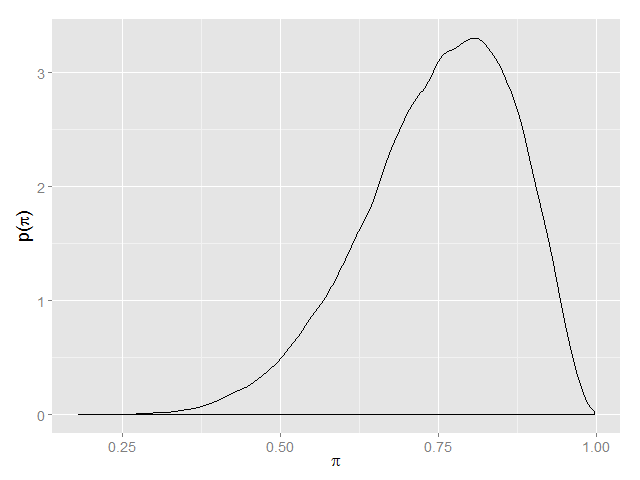
\includegraphics[width=\textwidth]{mainmatter/chapter_2_bayesian_paradigm/beta_prior.png}
        \caption{Prior $p(\pi)$: $\beta(9,3)$}
        \label{subfig : toy_problem_prior}
	\end{subfigure}
    	\begin{subfigure}[b]{0.45\textwidth}
		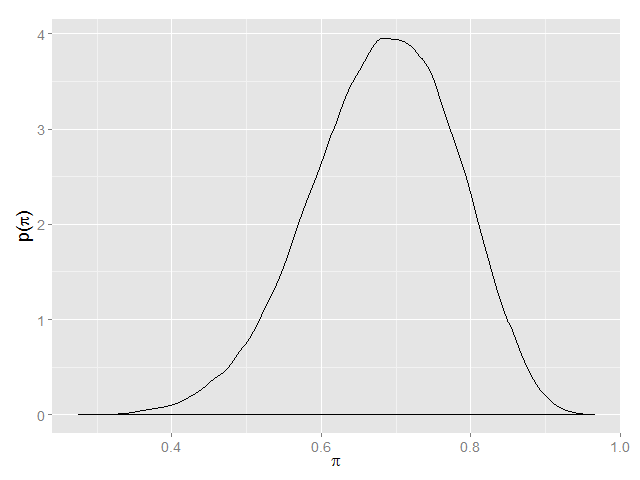
\includegraphics[width=\textwidth]{mainmatter/chapter_2_bayesian_paradigm/beta_posterior.png}
        \caption{Posterior $p(\pi|\boldsymbol{y})$: $\beta(15,7)$}
        \label{subfig : toy_problem_posterior}
	\end{subfigure}
\caption{Prior and posterior PDF for $\pi$; the probability of getting heads.}
\end{figure}

While subjective, these beliefs represent the prior probability distribution of a random variable in Bayesian paradigm. In our toy problem the random variable is probability $\pi$ of getting a heads. For e.g. in figure \ref{subfig : toy_problem_prior} we can see one such prior distribution corresponding to the belief that the chance of getting a heads on toss is more than tails and it is more likely to be somewhere between 70 to 90\%. This is in contrast to the frequentist paradigm where parameters do not have a distribution but are rather constants. Also the point and interval estimation in frequentist paradigm do not take prior beliefs into account and rely completely on the data at hand. While a detailed discussion of Bayesian vs. Frequentist approaches can be found in \citet{lesaffre_bayesian_2012}, we will present a brief overview of Bayes theorem and its usage in Bayesian parameter estimation.\\

\section{Bayes theorem}
\label{sec : bayes_theorem}
To understand the use of Bayes theorem in parameter estimation let us first look at one of the frequentist approach Maximum likelihood estimation to estimate the probability of getting heads ($\pi$). Suppose after 10 matches captain B observed that 6 times out 10 the toss resulted in heads. Assuming that conditions in each toss were such that the tosses were independent, then based on the likelihood function $L(\pi|\boldsymbol{y})$ the MLE of $\pi$ will be $\hat{\pi} = 0.6$. In contrast, the Bayes rule provides the framework to estimate the entire distribution of $\pi$ based on the data and the prior beliefs. The bayes rule for the continuous parameter $\pi$ is given by\\

\begin{equation}
\label{eq : bayes_rule}
p(\pi|\boldsymbol{y}) = \dfrac{L(\pi|\boldsymbol{y})p(\pi)}{p(\boldsymbol{y})} = \dfrac{L(\pi|\boldsymbol{y})p(\pi)}{\int_{0}^{1}L(\pi|\boldsymbol{y})p(\pi)d\pi}
\end{equation}

The result $p(\pi|\boldsymbol{y})$ is called the posterior distribution of the parameter based on which statistical inference about the parameter can be done. An intuitive way to get the motivation behind the bayes theorem is that the denominator can be seen as marginal probability of $\boldsymbol{y}$ based on the law of total probability. This is more evident in the categorical case though. In figure \ref{subfig : toy_problem_posterior} we can see the posterior PDF for the probability of getting heads that we obtained after applying Bayes rule. The mean value of this distribution is 0.7 which if you compare with the MLE of 0.6 you can see that Bayesian posterior mean is influenced by the prior as well.\\
\todo[inline]{The intuition part is needed to be expanded upon, and shall I talk of CI at this moment???}

\section{Bayesian software}
We can see in equation \ref{eq : bayes_rule} that the computation of posterior involves solving the integral in the denominator. While the calculations are simple in certain cases, for e.g. in exponential family the choice of conjugate prior leads to a posterior belonging to the same family. However it also depends on the prior beliefs. For e.g. if the prior belief for $\pi$ in our toy example is that it is trimodal then we may have to use numerical approximation for calculation of the posterior. The most widely used algorithms for posterior approximation are Markov chain monte carlo (MCMC) techniques like Gibbs sampling, Slice sampling, Metropolis hastings and their variants etc.\\

The software tools we will use are from the BUGS family like JAGS or WinBUGS. While WinBUGS provides its own integrated development environment it definitely lacks the usability and visualization capabilities offered in R. JAGS on the other hand relies on third party tools completely for visualization and analysis of MCMC chains. There are R packages namely R2jags, R2WinBUGS which allow users to execute JAGS/WinBUGS code via R. For Bayesian linear mixed models the R package blme will be used. For bayesian mixture models we will evaluate the R package bayesmix. The R package coda provides a rich array of functions to do analysis and diagnosis of MCMC chains.\\